% !TEX encoding = UTF-8
% !TEX TS-program = pdflatex
% !TEX root = ../tesi.tex

%**************************************************************
\chapter{Progettazione e codifica}
\label{cap:progettazione-codifica}
%**************************************************************

\intro{Il capitolo descrive in dettaglio la struttura del progetto, la progettazione e codifica delle nuove funzionalità, nonchè l'integrazione di esse con la struttura preesistente. Le fasi di progettazione e codifica non sono intese come attività prettamente distinte, infatti alcune analisi effettuate durante la progettazione iniziale antecedente alla codifica sono risultate non sufficienti a coprire numerose casistiche sorte durante lo sviluppo effettivo, per cui è stato necessaria una riprogettazione mirata a risolvere le problematiche sorte.}

%\section{Adattamento degli operatori preesistenti}
%Durante l'analisi preventiva dei rischi relativa alle nuove funzionalità, sono sorti dei problemi architetturali relativi %all'adattabilità degli operatori preesistenti con le nuove funzionalità create. Tali problematiche di adattabilità si possono %riassumere in micro-aree:

%\begin{itemize}
%	\item{adattabilità della rappresentazione degli eventi tramite l'\textit{output} dell'\textbf{operatore \textit{Bumblebee}} %definito come \textbf{\textit{BumblebeeOutput}}, che va a definire la trasformazione degli eventi "grezzi" in eventi arricchiti %con informazioni necessarie per il loro processamento;}
%	\item{adattabilità dell'\textbf{operatore \textit{Windowing}} che ora non deve solo trattare aggregazione di eventi ricevuti %dallo stesso tipo di risorsa, ma deve gestire l'aggregazione e/o l'allineamento anche di risorse di tipo differente per permettere %all'operatore \textit{AlertCoProcess} di eseguire un controllo a livello di insieme relativo a risorse differenti;}
%	\item{adattabilità dell'\textbf{operatore \textit{AlertCoProcess}} per permettere ad esso di gestire e di controllare gruppi di %eventi derivanti da risorse non più eguali fra di loro. Quindi di gestire il controllo relativo alla presenza di una anomalia %relativa ad un gruppo di risorse.}
%\end{itemize}
	
%Nello specifico si va ad analizzare le soluzioni proposte, nonchè la codifica effettiva, riguardo i problemi architetturali appena %descritti.

%**************************************************************

\section{Architettura componente anomaly detection}
In tale paragrafo si va ad evidenziare come le parti della componente di \textit{anomaly detection} interagiscono fra di loro. Come descritto nei capitoli precedenti, la componente realizzata tratta dapprima il raggruppamento degli eventi provenienti da determinate risorse secondo una finestra temporale, in seguito viene svolta un'analisi relativa a se tale insieme di eventi produce un'anomalia.
L'architettura rappresentante la componente di \textit{anomaly detection} è descritta tramite un \gls{diagramma delle classi}, il quale espone le seguenti strutture dati:
\begin{itemize}
	\item{\textbf{\textit{GroupedEvents}:} classe rappresentante i dati aggregati per uno specifico gruppo (\S\ref{sec:ge});}
	\item{\textbf{\textit{BboutAggregator}:} classe che si occupa di aggregare/allineare gli \textit{asset} entranti nella finestra temporale (\S\ref{sec:aggregator});}
	\item{\textbf{\textit{Windowing}:} classe rappresentante l'operatore che gestisce l'aggregazione dei dati su una finestra temporale (\S\ref{sec:windowing});}
	\item{\textbf{\textit{AlertCoProcess}:} classe rappresentante l'operatore che si occupa del rilevamento di anomalie (\S\ref{sec:alertcoprocess});}
	\item{\textbf{\textit{KeyedCoProcessFunction}:} classe astratta offerta da \textit{Flink}, da cui ereditano i due operatori citati precedentemente.}
\end{itemize}
All'interno del diagramma, per semplicità, vengono citate ma non descritte tutte le strutture dati con cui le classi operano, questo perchè tali strutture non risultano modificate durante la realizzazione del progetto e mantengono le funzionalità preesistenti. Inoltre le classi \textit{BumblebeeOutput} e \textit{AnomalyStepConfigurationCommand} vengono omesse perchè rappresentano semplicemente la struttura di due tipi di eventi entranti descritti rispettivamente nelle sezioni \S\ref{sec:bbout} e \S\ref{sec:api-configurazione}.
Di seguito la rappresentazione del diagramma appena descritto.

\begin{figure}[H] 
    \centering 
    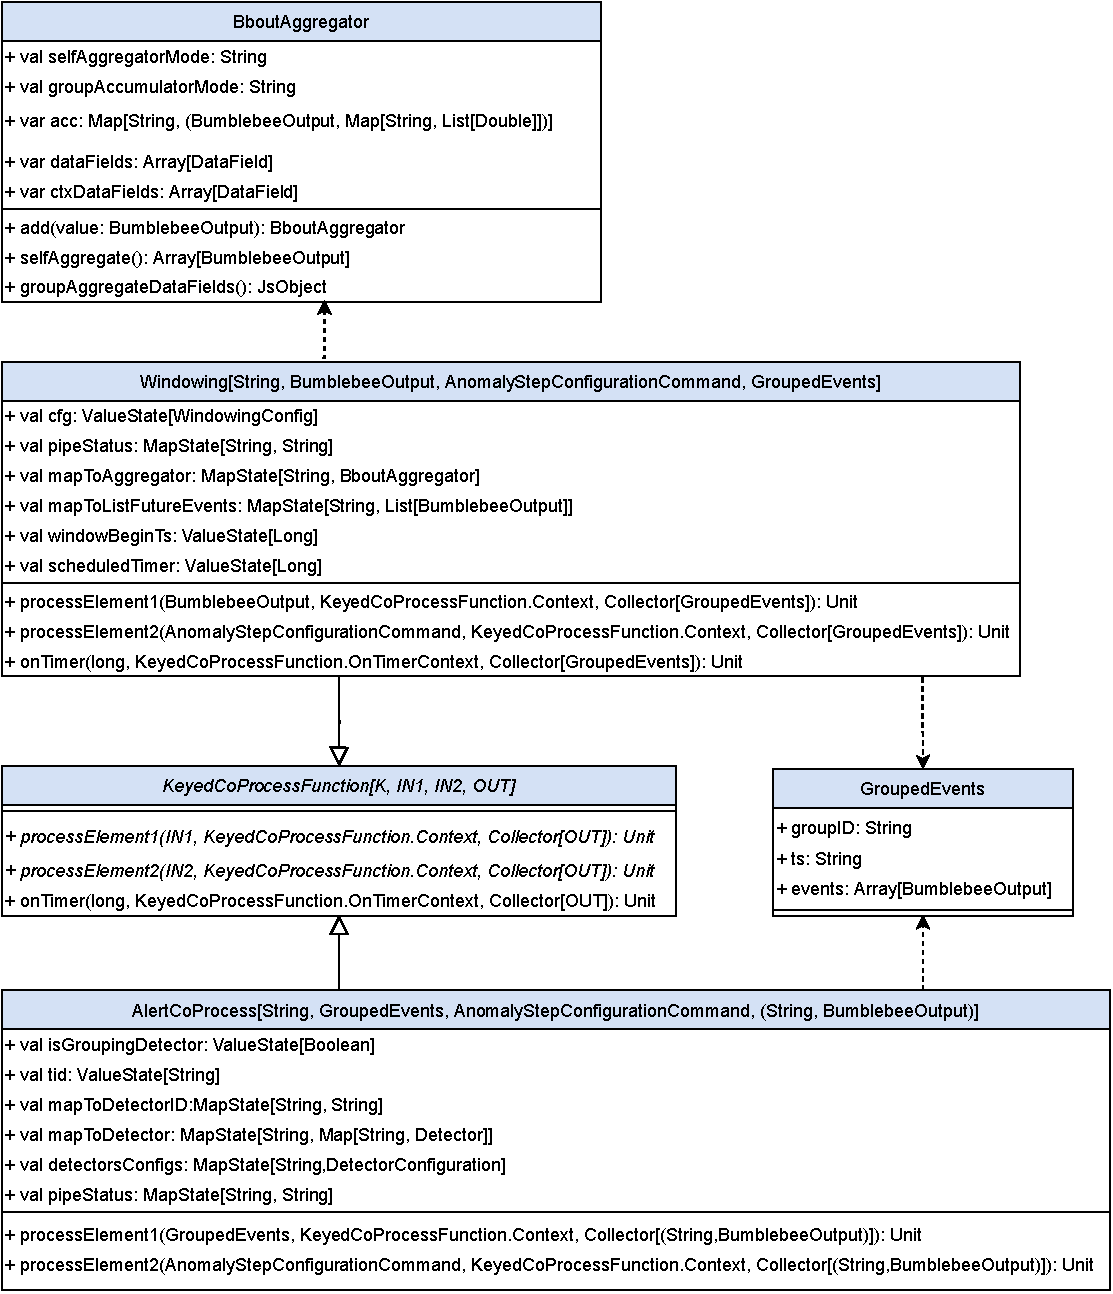
\includegraphics[width=1\columnwidth]{diagrammaClassi/anomaly_detection} 
    \caption{Diagramma delle classi componente \textit{anomaly detection}}
\end{figure}

\section{Classe GroupedEvents}\label{sec:ge}
\begin{figure}[H] 
    \centering 
    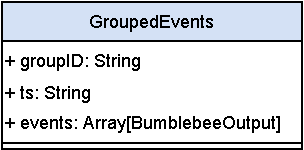
\includegraphics[width=0.4\columnwidth]{diagrammaClassi/groupedEventsClass} 
    \caption{Classe \textit{GroupedEvents}}
\end{figure}
La classe rappresentante un gruppo di eventi raggruppati è denominata \textit{GroupedEvents}. Dapprima tale struttura rappresentava solo una \textbf{risorsa singola}, ora invece tratta un \textbf{gruppo}, il quale è identificato da:
\begin{itemize}
	\item{\textbf{\textit{groupID}:} \textit{id} identificativo del gruppo;}
	\item{\textbf{\textit{ts}:} \textit{\gls{timestamp}} dell'evento raggruppato;}
	\item{\textbf{\textit{events}:} \textit{array} di risorse di tipo \textit{BumblebeeOutput}.}
\end{itemize}
\textit{GroupedEvents} può rappresentare logicamente due tipi logici di dato:
\begin{itemize}
	\item{\textbf{singolo elemento aggregato:} dove l'\textit{array} degli eventi è formato da un singolo elemento (aggregato su se stesso), l'\textit{id} del gruppo equivale all'\textit{id} definito dalla configurazione e il \textit{\textit{\gls{timestamp}}} equivale a quello definito durante l'aggregazione effettiva;}
	\item{\textbf{allineamento:} dove l'\textit{array} degli eventi è formato da \textit{N} elementi, l'\textit{id} del gruppo equivale all'\textit{id} definito dalla configurazione e il \textit{\textit{\gls{timestamp}}} equivale a quello definito durante l'aggregazione effettiva. L'allineamento è inteso come raggruppamento di eventi differenti che verranno analizzati a livello d'insieme.}
\end{itemize}

\section{Classe BboutAggregator}\label{sec:aggregator}
\begin{figure}[H] 
    \centering 
    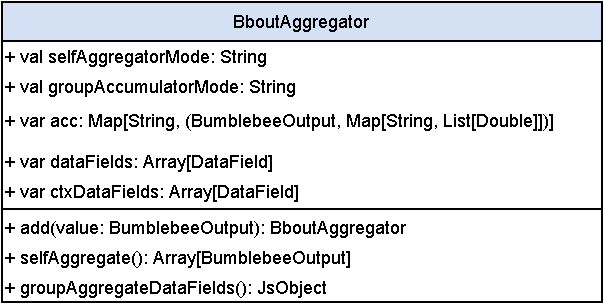
\includegraphics[width=0.7\columnwidth]{diagrammaClassi/bboutAggregatorClass} 
    \caption{Classe \textit{BboutAggregator}}
\end{figure}
\textit{BboutAggregator} è la componente che si occupa di aggregare o allineare gli eventi all'interno della finestra temporale. L'aggregatore in questione è una classe contenente i seguenti parametri:

\begin{itemize}
	\item{\textbf{\textit{selfAggregatorMode}:} definisce il tipo di aggregazione che verrà fatto sugli eventi dello stesso \textit{asset};}
	\item{\textbf{\textit{groupAccumulatorMode}:} definisce il tipo di aggregazione che verrà eseguito su \textit{asset} all'interno dello stesso gruppo;}
	\item{\textbf{\textit{acc}:} struttura che gestisce la mappatura fra un particolare \textit{asset} e una mappa che per chiave ha il nome di uno specifico parametro su cui si vuole andare a fare l'aggregazione e per valore ha la lista dei valori di quel parametro visti fino a quel determinato momento;}
	\item{\textbf{\textit{dataFields}:} \textit{array} contente i parametri degli eventi su cui si vuole fare l'aggregazione, decisi all'interno della \textbf{configurazione della \textit{window}};}
	\item{\textbf{\textit{ctxDataFields}:} \textit{array} contente i parametri del contesto degli eventi su cui si vuole fare l'aggregazione, decisi all'interno della \textbf{configurazione della \textit{window}}}
\end{itemize}

I metodi principali che gestiscono l'aggregazione a livello di \textbf{\textit{asset}} e a livello di \textbf{gruppo} sono:

\begin{itemize}
	\item{\textbf{\textit{add}:} tale metodo si occupa di salvare i valori dei parametri relativi agli eventi entranti nell'operatore \textit{Windowing}, dove tali parametri sono la concatenazione di \textit{dataFields} e \textit{ctxDataFields}. Per cui ad ogni chiamata di tale metodo verrà passato un particolare evento di tipo \textit{BumblebeeOutput}, tramite l'\textit{id} dell'evento viene estratta la mappa corrispondente ai parametri di \textit{dataFields} e \textit{ctxDataFields} e verrà aggiunto il valore del determinato parametro alla \textbf{lista dei valori} se esso è contenuto all'interno dell'evento.\\
Alla fine viene aggiornato il parametro \textit{acc} con la mappa aggiornata contenente la lista dei valori arricchita del nuovo valore, se trovato;}
	\item{\textbf{\textit{selfAggregate}:} tale metodo si occupa della vera e propria aggregazione degli \textbf{eventi provenienti dallo stesso \textit{asset}}, cioè per ogni evento all'interno della mappa \textit{acc} (dove l'\textit{asset} è la chiave stessa) verranno aggregati i valori contenuti nel parametro \textit{dataFields} e \textit{ctxDataFields} secondo il metodo di aggregazione definito da \textit{selfAggregatorMode}.\\
	Se un determinato parametro ha la lista dei rispettivi valori minore o uguale a zero, vuol dire che esso non è appartenuto allo specifico \textit{BumblebeeOutput} che si sta aggregando, perciò tale parametro \textbf{non} verrà aggiunto con un valore di default durante l'aggregazione.\\
	Come tipo di ritorno tale metodo ritornerà un \textit{array} di \textit{BumbleebeeOutput} dove ogni \textit{asset} avrà i parametri interni a \textit{dataFields} e \textit{ctxDataFields} aggregati secondo il metodo definito e i parametri non interni ai due \textit{array} appena citati valorizzati con l'ultimo elemento visto di quel parametro. Se un determinato \textbf{asset} non contiene nessun \textit{dataField}, non viene aggiunto all'\textit{array} ritornato;}
	\item{\textbf{\textit{groupAggregateDataFields}:} tale metodo si occupa di aggregare i parametri all'interno di \textit{asset} diversi fra di loro, aggregati precedentemente su se stessi tramite il metodo \textit{selfAggregate}. Per ogni parametro contenuto nell'\textit{array dataFields} viene fatta l'aggregazione di esso solo se presente come parametro all'interno degli eventi di tipo \textit{BumblebeeOutput} ritornati dal metodo \textit{selfAggregate}. Il metodo ritorna un \textit{\gls{json}} contenente l'aggregazione dei parametri contenuti in \textit{dataFields} secondo il metodo definito in \textit{groupAccumulatorMode}. Se un determinato parametro non è contenuto in almeno un \textit{BumblebeeOutput}, viene ritornato un \textit{\gls{json}} vuoto, per permettere all'operatore di \textit{Windowing} di poter saltare l'emissione del \textit{groupedEvents} che verrebbe creato.}
\end{itemize}
  


%**************************************************************

\section{Operatore Windowing}\label{sec:windowing}
\begin{figure}[H] 
    \centering 
    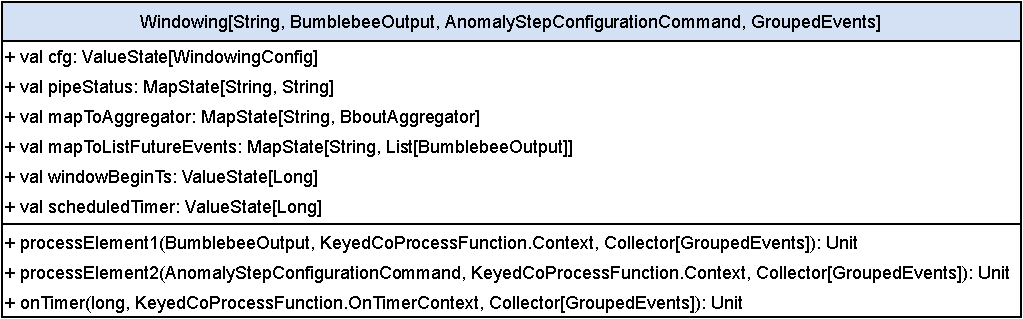
\includegraphics[width=0.9\columnwidth]{diagrammaClassi/windowingClass} 
    \caption{Classe \textit{Windowing}}
\end{figure}
L'\textbf{operatore \textit{Windowing}} serve per rappresentare un determinato evento in una data finestra temporale. Inizialmente, tale operatore, trattava l'aggregazione solo di una determinata \textbf{risorsa} su se stessa, cioè \textbf{sommando} o \textbf{mediando} un determinato valore. Ora in tale operatore non solo permane il comportamento appena descritto, ma è presente anche la funzionalità che si occupa di allineare/aggregare fra di loro eventi di \textit{asset} differenti, per permettere un'elaborazione dei dati a livello collettivo. Per definire il comportamento della finestra temporale, è necessaria un'apposita \textbf{configurazione} che sarà iniettata durante l'elaborazione attiva dei dati, per permetterne la modifica del comportamento senza dover riavviare l'intero applicativo e creare uno stallo in esso.\\
L'operatore \textit{Windowing} è una \textbf{\textit{KeyedCoProcessFunction}}, così definita:
\begin{minted}{scala}
class Windowing(outputTagValues: OutputTag[AnomalyStepConfigurationCommand]) extends KeyedCoProcessFunction[String, BumblebeeOutput, AnomalyStepConfigurationCommand, GroupedEvents] {
	// ...
  }
\end{minted}
Dove in entrata avrà due tipi di flussi, uno relativo agli eventi da raggruppare di tipo \textit{BumblebeeOutput} (\S\ref{sec:pr1-windowing}) e uno relativo alla configurazione dell'operatore di tipo \textit{AnomalyStepConfigurationCommand} (\S\ref{sec:pr2-windowing}). Tale operatore opera su flussi suddivisi per chiave definita come \textit{pipeID}.\\
Il metodo che verrà richiamato alla fine di una specifica finestra temporale è il metodo \textit{onTimer} (\S\ref{sec:on-timer-windowing}), il quale collezionerà gli eventi all'interno della \textit{window} appena conclusa e programmerà l'inizio della successiva finestra temporale.

\subsection{Stati dell'operatore}\label{sec:stati-windowing}
Per permettere una corretta gestione di entrambi i flussi, l'operatore \textit{Windowing} sfrutta i seguenti \textbf{stati} interni:
\begin{itemize}
		\item{\textbf{\textit{cfg}:} l'attuale configurazione della finestra temporale;}
		\item{\textbf{\textit{mapToAggregator}:} mappa che gestisce gli aggregatori (\S\ref{sec:aggregator}), i quali sono mappati per l'\textit{id} del gruppo;}
		\item{\textbf{\textit{mapToListFutureEvents}:} mappa che gestisce la lista degli eventi arrivati in anticipo, i quali sono mappati per l'\textit{id} del gruppo;}
		\item{\textbf{\textit{windowBeginTs}:} l'inizio dell'attuale finestra temporale;}
		\item{\textbf{\textit{scheduledTimer}:} \textit{timer} schedulato per collezionare gli eventi visti dalla \textit{window}, il quale coincide con la fine dell'attuale finestra temporale;}
		\item{\textbf{\textit{pipeStatus}:} mappa che gestisce la versione delle varie \textit{\gls{pipeline}}, le quali sono mappate per l'\textit{id} della \textit{\gls{pipeline}}.}
\end{itemize}


\subsection{Flusso degli eventi da raggruppare}\label{sec:pr1-windowing}
Tale flusso è gestito dal metodo \textit{processElement1}, il quale è un metodo ereditato dalla classe \textbf{KeyedCoProcessFunction} e sovrascritto dalla classe rappresentante l'operatore (\textit{Windowing}). Gli \textit{step} previsti per la gestione del suddetto sono:

\begin{enumerate}
	\item{arrivo dell'evento di tipo \textit{BumblebeeOutput};}
	\item{si controlla se la configurazione sia presente, e nel caso in cui non lo sia, si saltano i passaggi successivi e l'evento viene ignorato;}
	\item{nel caso in cui l'evento sia contenuto all'interno del filtro di aggregazione della \textit{window}, verrà controllato che il determinato gruppo sia configurato per raggruppare il tipo dell'evento in entrata;}
\item{se l'evento è contenuto all'interno del filtro di un gruppo, viene controllato se la durata della \textit{window} è nulla (minore o uguale a zero), in questo caso l'evento viene memorizzato all'interno della struttura dati rappresentata dal \textit{GroupedEvents} (\S\ref{sec:ge}) senza essere aggregato o allineato con altri eventi. Il flusso relativo all'evento entrante termina.\\
Se, invece, la durata della \textit{window} è positiva (maggiore di zero), l'evento può essere inserito nell'attuale \textit{window} se il suo \textit{\gls{timestamp}} è compatibile con i limiti della suddetta (inizio e fine), oppure può essere inserito nello stato \textbf{\textit{mapToListFutureEvents}} (\S\ref{sec:stati-windowing}) così da essere trattato nella successiva finestra temporale, se ha un \gls{timestamp} successivo rispetto la fine dell'attuale finestra temporale.\\
Infine se il \gls{timestamp} dell'evento è antecendete l'inizio della \textit{window}, l'evento viene scartato.}
\end{enumerate}

Per gestire l'inizio di una determinata nuova finestra temporale (quindi basata su una nuova \textbf{configurazione} per essa) verrà fatto un controllo per definire se l'evento entrante è il primo a partire da una nuova configurazione. In questo caso l'inizio della \textit{window} è eguale al \textit{\gls{timestamp}} dell'evento entrante e la fine della \textit{window} è equivalente alla somma dell'inizio della finestra temporale con la sua durata (definita nella configurazione).
\subsection{Flusso di configurazione}\label{sec:pr2-windowing}
Tale flusso è gestito dal metodo \textit{processElement2}, ereditato dalla classe \textbf{KeyedCoProcessFunction} e sovrascritto dalla classe rappresentante l'operatore (\textit{Windowing}). Gli \textit{step} previsti per la gestione del suddetto sono:

\begin{enumerate}
	\item{arrivo dell'evento riguardate la configurazione di tipo \textit{AnomalyStepConfigurationCommand};}
	\item{si controlla se la configurazione è di tipo "\textit{update}" o "\textit{delete}", in caso contrario il flusso termina collezionando l'evento in un \textit{SideOutput}, cioè un coda differente rispetto a quella principale relativa ai \textit{GroupedEvents} (\S\ref{sec:ge}). Tale coda tratta gli eventi di tipo \textit{AnomalyStepConfigurationCommand}.\\
	Se la configurazione tratta uno dei due tipi citati precedentemente, viene controllata l'esistenza della configurazione relativa alla \textit{window}, contenuta all'interno della configurazione di tipo \textit{AnomalyStepConfigurationCommand}. In caso in cui la configurazione non sia presente, vengono svuotati tutti gli stati all'interno della sezione \S\ref{sec:stati-windowing}. Alternativamente, viene controllato che essa sia differente rispetto a quella precedente, il che significa che la precedente è inesistente oppure che si differenzia da quella attuale per almeno una di queste condizioni:
	\begin{itemize}
		\item{differente durata della finestra temporale;}
		\item{differente metodo di aggregazione;}
		\item{differente lista di gruppi su cui lavorerà la \textit{window};}
		\item{differenti parametri \textbf{relativi ai dati degli eventi} su cui si andrà a fare l'aggregazione;}
		\item{differenti \textbf{parametri del contesto} relativi agli eventi su cui si andrà a fare l'aggregazione.}
	\end{itemize}
	
	A questo punto, solo se la configurazione della \textit{window} è differente da quella precedente, vengono svuotati i relativi stati dell'operatore su cui opera la finestra temporale, quali \textbf{\textit{mapToAggregator}}, \textbf{\textit{mapToListFutureEvents}}, \textbf{\textit{windowBeginTs}} e \textbf{\textit{scheduledTimer}}. Di seguito viene aggiornato lo stato \textbf{\textit{cfg}} con i dati della nuova finestra temporale.\\
Infine, sia che la nuova finestra temporale sia eguale o diversa rispetto la precedente, viene aggiornato \textbf{\textit{pipeStatus}}.\\
Per una descrizione approfondita degli stati dell'operatore \textit{Windowing} fare riferimento alla sezione \S\ref{sec:stati-windowing}.}
\end{enumerate}

\subsection{OnTimer}\label{sec:on-timer-windowing}
Il metodo \textbf{\textit{onTimer}} gestisce la logica al termine di ogni finestra temporale. Tale funzione si occupa di creare un \textit{GroupedEvents} (\S\ref{sec:ge}) collezionando gli eventi visti secondo le regole definite dalla configurazione e ha il compito di configurare la prossima \textit{window}. Il metodo segue questi \textit{step}:
\begin{enumerate}
	\item{controllo relativo a se la configurazione della finestra temporale è settata, in caso negativo vengono saltati tutti gli \textit{step} successivi;}
	\item{in base alla modalità di aggregazione definita nella configurazione della finestra temporale, per ogni \textbf{\textit{id} del gruppo} contenuto all'interno dello stato \textbf{\textit{mapToAggregator}} verrà creato ed emesso un \textit{GroupedEvents} (\S\ref{sec:ge}) contenente gli eventi aggregati o allineati secondo la modalità definita, la quale può essere:
	\begin{itemize}
		\item{\textbf{\textit{barrier}:} in questa modalità gli eventi vengono \textbf{allineati} e il metodo che si occupa di questa funzionalità è il metodo \textit{selfAggregate} dell'aggregatore;}
		\item{\textbf{\textit{aggregation\textunderscore sum}:} in questa modalità gli eventi vengono raggruppati in uno unico, per cui verrà creato un nuovo \textit{BumblebeeOutput} che come parametri avrà il \textit{\gls{json}} ritornato dal metodo \textit{groupAggregateDataFields} dell'aggregatore;}
		\item{\textbf{\textit{aggregation\textunderscore mean}:} in questa modalità gli eventi vengono raggruppati in uno unico, per cui verrà creato un nuovo \textit{BumblebeeOutput} che come parametri avrà il \textit{\gls{json}} ritornato dal metodo \textit{groupAggregateDataFields} dell'aggregatore.}
	\end{itemize}
	Per la logica specifica di aggregazione vedere la sezione \S\ref{sec:aggregator};}
	\item{creazione della nuova finestra temporale, cui inizio e fine sono impostati rispettivamente con il \textit{\gls{timestamp}} che ha attivato il metodo \textit{onTimer} e tale \textit{\gls{timestamp}} sommato alla durata della \textit{window}. Di seguito vengono rimossi gli aggregatori all'interno dello stato \textbf{\textit{mapToAggregator}} che non contengono eventi inseriti nello stato \textbf{\textit{mapToListFutureEvents}} (nel caso in cui siano presenti degli eventi futuri, verrà istanziato un nuovo aggregatore contente già questi eventi). Infine viene svuotato lo stato \textbf{\textit{mapToListFutureEvents}}.
	}
\end{enumerate}





%**************************************************************
\section{Operatore AlertCoProcess}\label{sec:alertcoprocess}
\begin{figure}[H] 
    \centering 
    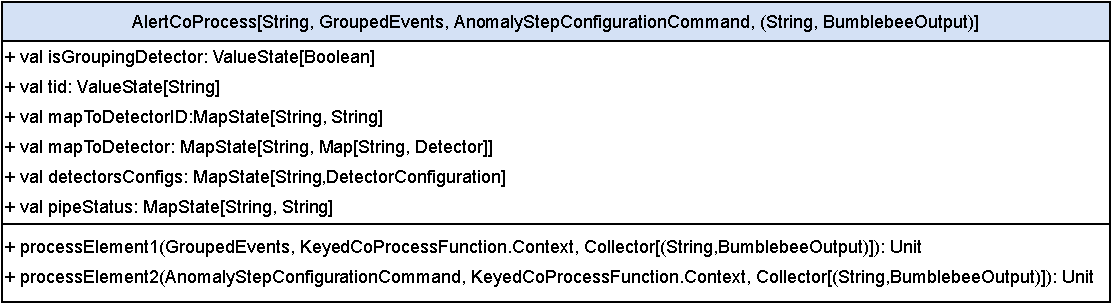
\includegraphics[width=0.9\columnwidth]{diagrammaClassi/alertCoProcessClass} 
    \caption{Classe \textit{AlertCoProcess}}
\end{figure}
L'operatore \textbf{\textit{AlertCoProcess}} si occupa di sollevare segnalazioni nel caso sia presente un'anomalia riguardo l'evento entrante di tipo \textit{GroupedEvents} (\S\ref{sec:ge}). Dapprima l'\textit{AlertCoProcess} lavorava solo su un tipo di evento legato ad una risorsa singola, mappando l'\textit{id} del \textit{detector} ad un'altra mappa dove la chiave veniva rappresentata dall'\textit{id} della risorsa e il valore veniva rappresentato dal vero e proprio \textit{detector}.\\
Ora, invece, la struttura è basata sull'\textit{id} del gruppo, per cui è stata creata un'ulteriore mappa fra \textit{id} del gruppo e \textit{id} del \textit{detector}, inoltre la chiave della mappa interna non è più rappresentata da un \textit{id} della risorsa, ma da un \textit{id} del soggetto dopo la modifica di \textit{Bumblebee} (\S\ref{sec:bbout}).\\
L'operatore \textit{AlertCoProcess} è una \textbf{\textit{KeyedCoProcessFunction}}, così definita:
\begin{minted}{scala}
class AlertCoProcess (inspectionTag: OutputTag[MongoInsertDocument]) extends KeyedCoProcessFunction[String, GroupedEvents, AnomalyStepConfigurationCommand, (String, BumblebeeOutput)] {
	// ...
  }
\end{minted}
Dove in entrata avrà due tipi di flussi: uno relativo agli eventi su cui controllare se viene rilevata un'anomalia di tipo \textit{GroupedEvents} (\S\ref{sec:pr1-alertcoprocess}) e uno relativo alla configurazione dell'operatore di tipo \textit{AnomalyStepConfigurationCommand} (\S\ref{sec:pr2-alertcoprocess}). Tale operatore opera su flussi suddivisi per chiave definita come \textit{pipeID}.\\
L'operatore lavora su un singolo tipo di \textit{detector}, il quale è legato indirettamente al \textit{pipeID}. Anche se il tipo di \textit{detector} è lo stesso, la configurazione dei parametri può cambiare a seconda del tipo di gruppo che viene definito all'interno del \textit{GroupedEvents} entrante.


\subsection{Stati dell'operatore}\label{sec:stati-alertcoprocess}
Per permettere una corretta gestione di entrambi i flussi, l'operatore \textit{AlertCoProcess} sfrutta i seguenti \textbf{stati} interni:
\begin{itemize}
		\item{\textbf{\textit{isGroupingDetector}:} valore \textit{booleano} che identifica se il \textit{detector} deve emettere l'evento come raggruppato oppure no;}
		\item{\textbf{\textit{tid}:} identifica il \textit{tenant} all'interno dell'\textit{AlertCoProcess};}
		\item{\textbf{\textit{mapToDetectorID}:} mappa che gestisce la correlazione fra l'\textit{id} del gruppo (chiave) e l'\textit{id} del \textit{detector} (valore);}
		\item{\textbf{\textit{mapToDetector}:} mappa che gestisce la correlazione fra il l'\textit{id} del \textit{detector} (chiave) e un ulteriore mappa (valore) che lega l'\textit{id} di un \textbf{soggetto}/\textbf{gruppo} con il suo vero e proprio \textit{detector};}
		\item{\textbf{\textit{detectorsConfigs}:} l'attuale configurazione del tipo di \textit{detector};}
		\item{\textbf{\textit{pipeStatus}:} mappa che gestisce la versione delle varie \textit{\gls{pipeline}}, le quali sono mappate per l'\textit{id} della \textit{\gls{pipeline}}.}
\end{itemize}

\subsection{Flusso degli eventi da analizzare}\label{sec:pr1-alertcoprocess}
Tale flusso è gestito dal metodo \textit{processElement1}, ereditato dalla classe \textbf{KeyedCoProcessFunction} e sovrascritto dalla classe rappresentante l'operatore (\textit{AlertCoProcess}). Gli \textit{step} previsti per la gestione del suddetto sono:
\begin{enumerate}
	\item{arrivo dell'evento di tipo \textit{GroupedEvents};}
	\item{viene estratta la mappa dei \textit{detector} tramite l'\textit{id} del \textit{detector}, ottenuto rispettivamente tramite l'\textit{id} del \textit{gruppo}. Ovviamente vengono effettuati dei controlli per verificare l'esistenza delle chiavi all'interno delle due mappe;}
	\item{se lo stato \textbf{\textit{isGroupingDetector}} ha come valore \textit{true}, vuol dire che l'anomalia, se presente, deve essere sollevata sul gruppo. Per cui viene estratto l'unico \textit{detector} (tramite l'\textit{id} del gruppo) dalla mappa estratta dallo \textit{step} precedente. Se il \textit{detector} è presente si utilizza quello preesistente, altrimenti ne viene creato uno nuovo. Infine viene creato un \textit{BumblebeeOutput} rappresentativo del gruppo su cui sollevare la possibile anomalia rilevata dal \textit{detector}.\\
	Se, altrimenti, lo stato \textbf{\textit{isGroupingDetector}} ha come valore \textit{false}, vuol dire che l'anomalia deve essere alzata su un singolo evento. Per cui per ogni evento interno all'\textit{array} degli eventi contenuto nell'oggetto \textit{GroupedEvents}, verrà estratto il \textit{detector} contenuto all'interno della mappa estratta nel punto 2. Anche in questa casistica viene creato un nuovo \textit{detector} se quelle estratto non esiste. In seguito viene controllato se il \textit{detector} è di tipo \textit{single input} (accetta un solo evento in entrata) oppure \textit{multiple input} (accetta un \textit{array} di eventi in entrata). A seconda dei due casi appena citati verrà passato o il singolo evento da cui si è estratto lo specifico \textit{detector} oppure tutto l'\textit{array} degli eventi. Nonostante ciò, la possibile anomalia verrà rilevata sull'evento a cui è mappato il \textit{detector}.}
\end{enumerate}

\subsection{Flusso di configurazione}\label{sec:pr2-alertcoprocess}
Tale flusso è gestito dal metodo \textit{processElement2}, ereditato dalla classe \textbf{KeyedCoProcessFunction} e sovrascritto dalla classe rappresentante l'operatore (\textit{AlertCoProcess}). Gli \textit{step} previsti per la gestione del suddetto sono:

\begin{enumerate}
	\item{arrivo dell'evento di tipo \textit{AnomalyStepConfigurationCommand};}
	\item{gestione della configurazione in base alla sua tipologia:
	\begin{itemize}
		\item{\textbf{\textit{update}:} in questo caso è richiesto l'aggiornamento dei \textit{detector}. Per ogni \textit{detector} contenuto all'interno della nuova configurazione viene verificato se l'\textit{id} corrispondente ad esso è presente all'interno dello stato \textbf{\textit{mapToDetectorID}}. Nel caso in cui l'\textit{id} sia contenuto all'interno della mappa verrà fatto l'accesso alla lista relativa di tutti i veri e propri \textit{detector} collegati a quel determinato \textit{id}. Per cui ogni \textit{detector} verrà aggiornato secondo la nuova configurazione fornita. La modalità di aggiornamento del \textit{detector} è specificata nella sezione \S\ref{sec:detector-alertcoprocess}.\\
		Nel caso in cui l'\textit{id} del \textit{detector} non sia contenuto all'interno della mappa, invece, viene creata una mappa vuota che verrà popolata nella funzione \textit{processElement1} (\S\ref{sec:pr1-alertcoprocess}). Infine vengono aggiornati i rispettivi stati che gestiscono la mappatura dei \textit{detector} (\textbf{\textit{mapToDetectorID}} e \textbf{\textit{mapToDetector}}) rimuovendo, se necessario, i \textit{detector} non più presenti;}
		\item{\textbf{\textit{delete}:} questo tipi di configurazione si occupa di svuotare gli stati relativi alla gestione dei \textit{detector}, quali \textbf{\textit{mapToDetectorID}} e \textbf{\textit{mapToDetector}}. Infine vengono svuotati gli stati \textbf{\textit{detectorsConfigs}} e \textbf{\textit{pipeStatus}};}
		\item{\textbf{\textit{inspect}:} tale configurazione permettere di ispezionare il comportamento effettivo dei \textit{detector} collezionando delle analitiche sullo stato dei modelli.}
	\end{itemize}}
\end{enumerate}


\subsection{Lista dei detector}\label{sec:detector-alertcoprocess}
In tale paragrafo vengono introdotti i \textit{detector} utilizzati all'interno dell'operatore \textit{AlertCoProcess}. Non trattando direttamente l'aggiornamento dei modelli utilizzati dai \textit{detector} durante il periodo di stage, verrà solo citato quali richiedano tale ricalcolo.\\
Di seguito la lista rappresentante i \textit{detector} utilizzati dall'\textit{AlertCoProcess}:
\begin{itemize}
	\item{\textbf{\textit{Uniseas}}: \textit{detector} che lavora singolarmente su un tipo di risorsa analizzando la sua \textit{\gls{stagionalita}}. Il suo aggiornamento non richiede un ricalcolo del modello non usando un algoritmo di \textit{\gls{Apprendimento automatico}};}
	\item{\textbf{\textit{Crosscorrel}}: \textit{detector} che lavora singolarmente su un tipo di risorsa e su un evento esterno ad essa (come per esempio il tempo metereologico), analizzando la correlazione tra variabili. Il suo aggiornamento non richiede un ricalcolo del modello non usando un algoritmo di \textit{\gls{Apprendimento automatico}};}
	\item{\textbf{\textit{Siblings}}: \textit{detector} che lavora singolarmente su un tipo risorsa valutando il suo andamento in funzione dell'andamento di altri \textit{N} \textit{asset}. Utilizza un algoritmo di \textit{\gls{Apprendimento automatico}} di tipo \textit{\gls{Apprendimento supervisionato}}. A differenza dei precedenti \textit{detector}, l'algoritmo richiede un ricalcolo del modello nel caso di una nuova configurazione.}
\end{itemize}

%**************************************************************

\section{Operatore Bumblebee}\label{sec:bbout}
Per permettere la rappresentazione di gruppi di risorse differenti su cui ora operano gli operatori \textit{Windowing} e \textit{AlertCoProcess}, viene cambiata la struttura dell'\textit{output} dell'operatore \textbf{\textit{Bumblebee}}, rappresentato inizialmente in un formato \textit{\gls{json}} così formato:

\begin{minted}{js}
{
  "id": // id dell'evento, generato o trasformato dall'evento originale, in formato String
  "pipeID": // id della pipeline, in formato String
  "pipeVersion": //versione della pipeline, in formato String
  "adapterID": //id dell'adattatore, in formato String
  "tid": //id del cliente, in formato String
  "assetID": //id della risorsa, in formato String
  "ts": //timestamp dell'evento, in formato String
  "asset": //informazioni relative alla risorsa dopo che è stata arricchita, in formato AssetInfo
  "data": //payload dei dati dell'evento trasformati in formato JSON
  "ctxData": //dati relativi al contesto, come per esempio il tempo metereologico, in formato JSON
  "meta": //metadati arricchiti dall'operatore di anomaly detection, in formato Option[EventMeta]
  "type": //tipo di BumblebeeOutput, in formato Option[String]
  "srcID": //id della fonte dell'evento in formato String
}
\end{minted}

Dopo l'opportuna modifica, la struttura rappresentante il \textbf{\textit{BumblebeeOutput}} risulta la seguente:

\begin{minted}{js}
{
  "id": // id dell'evento, generato o trasformato dall'evento originale, in formato String
  "pipeID": // id della pipeline, in formato String
  "pipeVersion": //versione della pipeline, in formato String
  "adapterID": //id dell'adattatore, in formato String
  "tid": //id del cliente, in formato String
  "subject": {
	  "id": //id dell'oggetto, in formato String
	  "type": //tipo dell'oggetto rapresentanto (asset,category,group), in formato String
  }
  "ts": //timestamp dell'evento, in formato String,
  "asset": //informazioni relative alla risorsa dopo che è stata arricchita, in formato AssetInfo
  "data": //payload dei dati dell'evento trasformati in formato JSON
  "ctxData": //dati relativi al contesto, come per esempio il tempo metereologico, in formato JSON
  "meta": //metadati arricchiti dall'operatore di anomaly detection, in formato Option[EventMeta]
  "type": //tipo di BumblebeeOutput, in formato Option[String]
  "srcID": //id della fonte dell'evento in formato String
}
\end{minted}
dove la rappresentazione è slegata da un \textit{asset} (risorsa) specifico. Per cui l'\textit{output} sarà adattato ad un \textbf{soggetto} generale, rappresentato da un proprio \textbf{\textit{id}} e da un suo \textbf{tipo}.
Tale struttura finale garantisce una corretta elaborazione del dato nel caso in cui si tratti di un evento singolo oppure di un raggruppamento.

%**************************************************************

\section{API della configurazione}\label{sec:api-configurazione}
Dopo le modifiche apportate agli operatori precedenti è richiesta una nuova definizione delle \textit{\gls{api}} di governo che gestiscono i messaggi che vanno a definire la configurazione dell'\textit{anomaly detection}, cioè la configurazione denominata \textit{AnomalyStepConfigurationCommand}, la quale racchiude le configurazioni relative all'operatore \textit{Windowing} e all'operatore \textit{AlertCoProcess}. La nuova definizione delle \textit{\gls{api}} consiste in:

\begin{itemize}
	\item{definizione della nuova struttura del messaggio in formato \textit{\gls{json}} contenente le configurazioni decise dall'utente;}
	\item{controllo relativo alla correttezza e consistenza dei dati passati dall'utente.}
\end{itemize}
Per semplicità la definizione del messaggio fornito dall'\textit{\gls{api}} viene suddiviso e analizzato in sezioni differenti per esplicitare al meglio la parte relativa all'operatore \textit{Windowing} e quella relativa ai \textit{detector} utilizzati all'interno dell'operatore \textit{AlertCoProcess}.




\subsection{JSON di configurazione dell'operatore Windowing}\label{sec:json-windowing}
La definizione della configurazione relativa all'operatore \textit{Windowing} è così rappresentata:

\begin{minted}{js}
"windowing":{
    "duration": //durata della finestra temporale in minuti, in formato Int
    "aggregationMethod": //tipo di aggregazione per asset eguali fra di loro (sum|mean), in formato String
    "windowingMode": //modalità di aggregazione a gruppi (barrier,aggregation_sum,aggregation_mean), in formato String
    "dataFields": //parametri caratterizzante gli asset
    [
      {
        "name": // nome del parametro in formato String
        "kind": // tipo del parametro (continuous|categorical), in formato String
      }
    ],
    "ctxDataFields": //parametri del contesto caratterizzante gli asset 
    [
      {
        "name":  // nome del parametro in formato String
        "kind": // tipo del parametro (continuous|categorical), in formato String
      }
    ],
    "assetFilters": { // filtri da applicare all'interno della finestra temporale
        "groupID": {
            "id": //id identificativo del gruppo (uguale al groupID), in formato String
            "filterGeos": // id relativi alla posizione geografica di un asset, in formato Array[String]
            "filterBfuncs": //id relativi ad una funzione, in formato Array[String]
            "filterCats": //id relativi alla categoria di un asset, in formato Array[String]
            "filteredAssetsIds": //id relativi agli asset, in formato Array[String]
        } 
    }
}
\end{minted}
Le principali informazioni aggiuntive introdotte nel formato \textit{\gls{json}} relativo alla configurazione della finestra temporale sono:
\begin{itemize}
	\item{\textbf{\textit{windowingMode}:} definizione della modalità di aggregazione su gruppi;}
	\item{\textbf{\textit{assetFilters}}: ora i filtri da applicare ad una finestra temporale sono mappati per l'\textit{id} del gruppo. Così facendo si permette di avere filtraggi differenti per gruppi differenti.}
\end{itemize} 


\subsection{JSON di configurazione dell'operatore AlertCoProcess}\label{sec:json-detectors}
La definizione della configurazione relativa ai \textit{detector} è così rappresentata:
\begin{minted}{js}
"detectors": [
   {
    "detectorID": // id del detector, in formato String
    "detectorType": // tipo del detector (siblings|uniseas|ctx_ad_cross), in formato String
    "parameters": {
		// parametri relativi al tipo di detector    
    },
    "assetFilters":{
      "id": //id identificativo del gruppo (uguale al groupID), in formato String
      "filterGeos": // id relativi alla posizione geografica di un asset, in formato Array[String]
      "filterBfuncs": //id relativi ad una funzione, in formato Array[String]
      "filterCats": //id relativi alla categoria di un asset, in formato Array[String]
      "filteredAssetsIds": //id relativi agli asset, in formato Array[String]
    }
   }
  ]
}
\end{minted}
La principale informazione aggiuntiva introdotta nel formato \textit{\gls{json}} relativo alla configurazione dei \textit{detector} è rappresentata dall'\textit{id} relativo al gruppo introdotto all'interno di \textit{assetFilters}. Tale \textit{id} permette una corretta mappatura del gruppo con l'\textit{id} del \textit{detector} all'interno dell'operatore \textit{AlertCoProcess}.\\
Si è deciso di non rappresentare la struttura relativa ai parametri che identificano il \textit{detector} (rappresentanti dal campo \textit{parameters}) perchè essi rimangono invariati anche dopo l'aggiunta delle nuove funzionalità e sono scollegate da essa.

\subsection{JSON configurazione anomaly detection}
Di seguito viene rappresentato il messaggio \textit{\gls{json}} di configurazione globale fornito dall'\textit{\gls{api}} che si occupa di definire la configurazione decisa dall'utente:

\begin{minted}{js}
{
  "ctype": // tipo della configurazione cui dipende la deserializzazione, in formato String
  "tid": //id del cliente, in formato String
  "pipeID": // id della pipeline, in formato String
  "pipeVersion": //versione della pipeline, in formato String
  "outputTopic": // tipo di topic dell'output, in formato String
  "isGrouping": // rappresenta se l'anomalia deve essere sollevata su un gruppo, in formato Boolean
  "detectors": // configurazione dei detectors, in fomato Array
  "windowing": // configurazione della finestra temporale
 }
\end{minted}
dove:
\begin{itemize}
	\item{\textbf{\textit{detectors}}: rappresenta un \textit{array} di configurazioni come descritto nella sezione \S\ref{sec:json-detectors}};
	\item{\textbf{\textit{windowing}}: rappresenta la configurazione della finestra temporale come descritto nella sezione \S\ref{sec:json-windowing}.}
\end{itemize}

Rispetto alla configurazione iniziale è stato introdotto il campo \textit{isGrouping}, che definisce se i \textit{detector} devono emettere l'evento anomalo come raggruppato oppure no.

\subsection{Correttezza e consistenza dei dati forniti dall'utente}
A fronte della modifica del messaggio di configurazione fornito alla componente di \textit{anomaly detection}, serve garantire che i dati forniti dall'utente siano corretti e consistenti fra di loro.\\
Di seguito verrà descritto il controllo effettuato per garantire che la configurazione fornita sia corretta secondo le specifiche e secondo la configurazione preesistente nel caso si tratti di un aggiornamento.\\
Dopo la ricezione dei dati forniti dall'utente viene effettuato il seguente controllo:
\begin{itemize}
	\item{\textbf{verifica della consistenza della nuova configurazione:}
		\begin{enumerate}
			\item{si verifica che la lunghezza della mappa \textit{windowing.assetFilters} sia eguale alla lunghezza dell'\textit{array} \textit{detectors};}
			\item{per ogni elemento all'interno della mappa \textit{windowing.assetFilters} si verifica che la chiave dell'elemento (\textit{groupID}) sia corrispondente al campo \textit{id} contenuto dall'elemento stesso;}
			\item{per ogni elemento all'interno della mappa \textit{windowing.assetFilters} si verifica che tale elemento sia contenuto all'interno dell'\textit{array} \textit{detectors}.}
		\end{enumerate}}
	\item{\textbf{verifica della consistenze della nuova configurazione relativamente a quelle preesistente:} per ogni chiave della mappa \textit{windowing.assetFilters}, preesistente nella vecchia configurazione, viene verificato che il valore di tale mappa sia rimasto invariato rispetto alla precedente configurazione.}
\end{itemize}

Per ogni nuovo gruppo viene sostituito l'\textit{id} fornito dall'utente, richiesto per identificare la correlazione fra l'\textit{assetFilters} del gruppo contenuto all'interno della mappa \textit{windowing.assetFilters} e il medesimo \textit{assetFilters} contenuto nell'\textit{array} \textit{detectors}, con un \textit{id} appositamente creato dall'\textit{\gls{api}}.\\
Per ogni controllo appena elencato viene fornito un messaggio d'errore all'utente in caso di fallimento, questo per comunicare che tale configurazione non è corretta.


